% Faithful native paths from source/普通高考/2021/2021全国乙理(河南,山西,江西,安徽,陕西,甘肃,青海,内蒙古,黑龙江,吉林,.宁夏,新疆).pdf, page 1.
% Original outlines, connected rock fissures, solid/dashed edges and shaded regions retained.
% Labels retain their original objects; no arbitrary geometric substitute or raster wrapper.
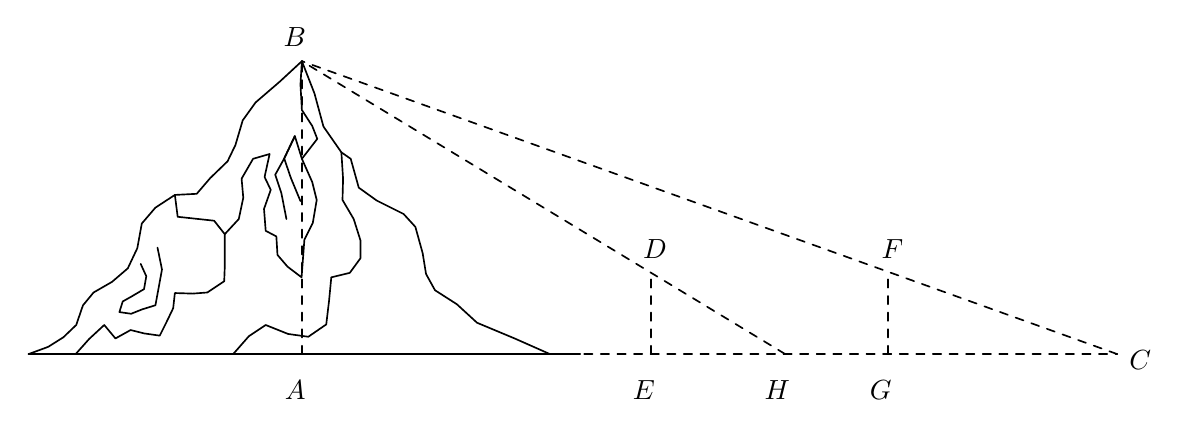
\begin{tikzpicture}[x=1cm,y=1cm,font=\normalsize,line join=round,line cap=round]
\path[draw=black,line width=0.6pt] (0.36972,0.83196) -- (0.61890,0.92372) -- (0.81110,1.04478) -- (0.97487,1.20138) -- (1.06028,1.45056) -- (1.19556,1.61433) -- (1.43052,1.74961) -- (1.62988,1.92049) -- (1.75089,2.17678) -- (1.80787,2.49004) -- (1.98099,2.69198) -- (2.22798,2.85318) -- (2.50565,2.86739) -- (2.67647,3.06676) -- (2.89722,3.28034) -- (2.99684,3.48681) -- (3.08942,3.80013) -- (3.25319,4.02793) -- (3.55934,4.29138) -- (3.84106,4.55199) -- (4.00078,4.14183) -- (4.11468,3.72178) -- (4.34248,3.39424) -- (4.46102,3.31200) -- (4.56322,2.94575) -- (4.79108,2.78198) -- (5.13278,2.61110) -- (5.28233,2.44734) -- (5.37490,2.11275) -- (5.41761,1.84929) -- (5.53151,1.64282) -- (5.80917,1.46484) -- (6.06546,1.22987) -- (6.54250,1.03056) -- (6.99104,0.83196) ;
\path[draw=black,line width=0.6pt] (0.96777,0.83196) -- (1.13865,1.02340) -- (1.33085,1.20138) -- (1.47324,1.03056) -- (1.66549,1.13730) -- (1.83637,1.09459) -- (2.03574,1.06610) -- (2.12115,1.23704) -- (2.20656,1.41502) -- (2.22794,1.60722) -- (2.45579,1.60012) -- (2.64088,1.61433) -- (2.85447,1.75672) -- (2.86158,1.94187) -- (2.86158,2.11275) -- (2.86158,2.35476) -- (2.72635,2.52569) -- (2.46290,2.55418) -- (2.26353,2.57551) -- (2.22794,2.85318) ;
\path[draw=black,line width=0.6pt] (1.79363,1.97745) -- (1.86482,1.82084) -- (1.83633,1.65708) -- (1.67972,1.56450) -- (1.56583,1.50047) -- (1.52312,1.36514) -- (1.67262,1.34376) -- (1.81500,1.40073) -- (1.98102,1.45197) -- (2.06418,1.90626) -- (2.00726,2.18392) ;
\path[draw=black,line width=0.6pt] (2.86158,2.35478) -- (3.03957,2.54704) -- (3.09654,2.81760) -- (3.07522,3.05962) -- (3.22105,3.31202) -- (3.43113,3.37294) -- (3.36710,3.08105) -- (3.44541,2.91728) -- (3.35994,2.67516) -- (3.38132,2.39749) -- (3.51665,2.32629) -- (3.53087,2.09133) -- (3.65899,1.94189) -- (3.83703,1.80661) -- (3.87257,2.28359) -- (3.97942,2.49723) -- (4.02923,2.78911) -- (3.97225,3.01691) -- (3.84102,3.31202) -- (3.75156,3.60073) -- (3.61628,3.31596) -- (3.50238,3.10948) -- (3.58069,2.87452) -- (3.64477,2.54704) ;
\path[draw=black,line width=0.6pt] (3.84104,4.55200) -- (3.82277,4.25574) -- (3.84104,3.93198) -- (3.97227,3.72889) -- (4.03636,3.56518) -- (3.84104,3.31201) ;
\path[draw=black,line width=0.6pt] (2.96839,0.83196) -- (3.16770,1.05900) -- (3.38134,1.20138) -- (3.66612,1.08749) -- (3.92246,1.05189) -- (4.15026,1.20855) -- (4.18586,1.50754) -- (4.21434,1.80659) -- (4.44931,1.86357) -- (4.58459,2.04866) -- (4.58459,2.27651) -- (4.49912,2.54702) -- (4.35673,2.78909) -- (4.36390,3.05965) -- (4.34252,3.39424) ;
\path[draw=black,line width=0.6pt] (3.75159,3.60074) -- (3.61631,3.31596) -- (3.70172,3.06678) -- (3.82278,2.77490) ;
\path[draw=black,line width=0.6pt] (0.36901,0.83196) -- (7.37506,0.83196) ;
\path[draw=black,line width=0.6pt,dash pattern=on 3pt off 3pt] (14.19515,0.83196) -- (3.84106,4.55199) ;
\path[draw=black,line width=0.6pt,dash pattern=on 3pt off 3pt] (9.97910,0.83196) -- (3.84104,4.55199) ;
\path[draw=black,line width=0.6pt,dash pattern=on 3pt off 3pt] (8.27407,0.83196) -- (8.27407,1.88599) ;
\path[draw=black,line width=0.6pt,dash pattern=on 3pt off 3pt] (11.28111,0.83196) -- (11.28111,1.88599) ;
\path[draw=black,line width=0.6pt,dash pattern=on 3pt off 3pt] (3.84104,0.83196) -- (14.19513,0.83196) ;
\path[draw=black,line width=0.6pt,dash pattern=on 3pt off 3pt] (3.84104,0.83196) -- (3.84104,4.55199) ;
\node[anchor=base west,inner sep=0pt,outer sep=0pt] at (3.62570,0.25448) {$A$};
\node[anchor=base west,inner sep=0pt,outer sep=0pt] at (3.60886,4.73719) {$B$};
\node[anchor=base west,inner sep=0pt,outer sep=0pt] at (14.35080,0.63577) {$C$};
\node[anchor=base west,inner sep=0pt,outer sep=0pt] at (8.17436,2.04210) {$D$};
\node[anchor=base west,inner sep=0pt,outer sep=0pt] at (11.20257,2.04210) {$F$};
\node[anchor=base west,inner sep=0pt,outer sep=0pt] at (8.04559,0.25448) {$E$};
\node[anchor=base west,inner sep=0pt,outer sep=0pt] at (9.71712,0.25448) {$H$};
\node[anchor=base west,inner sep=0pt,outer sep=0pt] at (11.05537,0.25448) {$G$};
\end{tikzpicture}
